\documentclass[conference]{IEEEtran}
\IEEEoverridecommandlockouts

\usepackage[
a4paper,
vmargin=2cm,
hmargin=1.5cm
]{geometry}

\usepackage{enumitem}
\usepackage[table]{xcolor}
\definecolor{azulUC3M}{RGB}{0,0,102}
\definecolor{gray97}{gray}{.97}
\definecolor{gray75}{gray}{.75}
\definecolor{gray45}{gray}{.45}

\usepackage[a-1b]{pdfx}
\usepackage{hyperref}
\hypersetup{colorlinks=true,
    linkcolor=black,
    urlcolor=blue}

\usepackage{amsmath,amssymb,amsfonts,amsthm}
\usepackage{newtxtext,newtxmath}
\usepackage[T1]{fontenc}
\usepackage[utf8]{inputenc}
\usepackage[english]{babel}
\usepackage[babel, english=american]{csquotes}
\AtBeginEnvironment{quote}{\small}

\usepackage{fancyhdr}
\pagestyle{fancy}
\fancyhf{}
\renewcommand{\headrulewidth}{0pt}
\rfoot{\thepage}
\fancypagestyle{plain}{\pagestyle{fancy}}

\usepackage{multirow}
\usepackage{caption}
\DeclareCaptionOption{compatibility}{false}
\usepackage{floatrow}
\usepackage{array}
\newcolumntype{P}[1]{>{\centering\arraybackslash}p{#1}}
\usepackage{graphicx}
\usepackage{float}
\graphicspath{{images/}}

\captionsetup*[table]{
    format=hang,
    name=Table,
    justification=centering,
    labelsep=period,
    width=\linewidth,
    labelfont=small,
    font=small
}

\captionsetup[figure]{
    format=hang,
    name=Fig.,
    justification=centering,
    singlelinecheck=off,
    labelsep=period,
    labelfont=small,
    font=small
}

\usepackage{chngcntr}
\usepackage{pdfpages}
\usepackage{listings}
\usepackage{xcolor}

\lstset{
    basicstyle=\ttfamily\small,
    breaklines=true,
    frame=single,
    backgroundcolor=\color{gray!5},
    keywordstyle=\color{blue},
    commentstyle=\color{green!60!black},
    stringstyle=\color{red},
    numbers=left,
    numberstyle=\tiny\color{gray},
    stepnumber=1,
    numbersep=5pt,
    showstringspaces=false
}

\lstdefinestyle{estilo}{
    frame=Ltb,
    framerule=0pt,
    aboveskip=0.5cm,
    framextopmargin=3pt,
    framexbottommargin=3pt,
    framexleftmargin=0.4cm,
    framesep=0pt,
    rulesep=.4pt,
    backgroundcolor=\color{gray97},
    rulesepcolor=\color{black},
    basicstyle=\ttfamily\footnotesize,
    keywordstyle=\bfseries,
    stringstyle=\ttfamily,
    showstringspaces=false,
    commentstyle=\color{gray45},
    numbers=left,
    numbersep=15pt,
    numberstyle=\tiny,
    numberfirstline=false,
    breaklines=true,
    xleftmargin=\parindent
}
\captionsetup*[lstlisting]{font=small, labelsep=period}
\lstset{style=estilo}

\usepackage[backend=biber, style=ieee, isbn=false, sortcites,
            maxbibnames=6, minbibnames=1]{biblatex}
\addbibresource{references.bib}

%-------------
%   DOCUMENT
%-------------

\begin{document}

%----------
%   COVER
%----------
\begin{titlepage}
    \begin{sffamily}
        \color{azulUC3M}
        \begin{center}
            \begin{figure}[H] % UC3M Logo
                \makebox[\textwidth][c]{
\includegraphics[width=16cm]{images/logo_UC3M.png}}
            \end{figure}
            \vspace{2.5cm}
            \begin{Large}
                Master's Degree in Cybersecurity\\
                2025-2026\\ % Academic year
                \vspace{2cm}
                \textsl{Master's Thesis}
                \bigskip

            \end{Large}
            {\Huge Multi-agent Architecture for IoT Threat Detection Using Language Models}\\
            \vspace*{0.5cm}
            \rule{10.5cm}{0.1mm}\\
            \vspace*{2cm}
            {\LARGE Author: María López Padilla}\\
            \vspace*{3cm}
            \begin{Large}
                Supervisors: \\
                Alfonso Alejandro Sánchez-Macián Pérez \\
                Pablo Mateo Torrejón \\
                \vspace*{1cm}
                Madrid, July 2026\\
            \end{Large}
        \end{center}
        \vfill
        \color{black}
        \fbox{
            \begin{minipage}{\linewidth}
                \textbf{AVOID PLAGIARISM}\\
                \footnotesize{The University uses the \textbf{Turnitin Feedback Studio} for the delivery of student work. This program compares the originality of the work delivered by each student with millions of electronic resources and detects those parts of the text that are copied and pasted. Plagiarizing in a TFM is considered a  \textbf{\underline{Serious Misconduct}}, and may result in permanent expulsion from the University.}\end{minipage}}

        % IF OUR WORK IS TO BE PUBLISHED UNDER A CREATIVE COMMONS LICENSE, INCLUDE THESE LINES. IS THE RECOMMENDED OPTION.
        \noindent
\includegraphics[width=4.2cm]{images/creativecommons.png}\\ % Creative Commons Logo
        \footnotesize{This work is licensed under Creative Commons \textbf{Attribution – Non Commercial – Non Derivatives}}

    \end{sffamily}
\end{titlepage}

%----------
%   PAPER
%----------

\title{Multi-agent Architecture for IoT Threat Detection Using Language Models}

\author{\IEEEauthorblockN{María López Padilla}
    \IEEEauthorblockA{\textit{Student}, \textit{Carlos III University}, Madrid, Spain\\
        100565051@alumnos.uc3m.es}
}

\maketitle

\begin{abstract}

    The growth of Internet of Things (IoT) devices has expanded the network attack surface. Supervised machine learning-based Intrusion Detection Systems (IDS) suffer from a cold start problem: when deployed in a network with an unseen telemetry schema, their accuracy degrades significantly. Operators are then forced to choose between running the network without protection or accepting service downtime while new data is collected and models are retrained.

    Our approach to this problem is a multi-agent architecture for IoT threat detection and automated incident response that keeps the system active throughout the entire cold start window. Schema mismatch is handled by a generative LLM agent performing zero-shot feature normalization, while a background thread simultaneously trains a schema-specific classifier and deploys it via a transparent hot-swap once it is ready. A separate Responder agent automates threat context generation and retrieves grounded mitigations from the MITRE CAPEC taxonomy via Retrieval-Augmented Generation (RAG).

    Tests on Edge-IIoTset, TON\_IoT, and Bot-IoT show that the universal fallback reaches 94.25\% binary accuracy during the cold start phase. After background training completes---in under 2.5 minutes---the hot-swap restores full multiclass classification at up to 96.68\% weighted F1-score with sub-5 ms inference latency. These results confirm that the fallback mode can sustain meaningful threat coverage without sacrificing long-term detection performance.
\end{abstract}

\vspace{0.5cm}

\begin{IEEEkeywords}
    IoT, intrusion detection, multi-agent architecture, large language models, high availability, zero downtime, cold start, XGBoost, RAG, MITRE ATT\&CK.
\end{IEEEkeywords}

%-----------
% SECTION 1
%-----------
\section{Introduction}
\label{sec:intro}

The Internet of Things (IoT) has grown rapidly over the last decade, with the number of active connected devices projected to reach 39 billion by 2030~\cite{iotanalytics2023}. While expanding industrial and consumer capabilities, this growth has significantly enlarged the network attack surface. Due to their limited computational resources, heterogeneous protocols, and lack of built-in security, IoT devices remain highly vulnerable and difficult to protect using traditional defense mechanisms.

Managing the security of these environments at scale has become a defining challenge for SOCs. Rather than consolidated, actionable intelligence, analysts receive floods of low-level, categorical alerts from conventional IDS tools---each one requiring manual investigation and triage. That volume is unsustainable: it drives alert fatigue, a well-documented state of cognitive overload in which genuine threats are buried under redundant notifications and false positives~\cite{paloalto2024alertfatigue}. The Cost of a Data Breach report~\cite{ibm2025cost} puts the average time to identify and contain a breach at 241 days, a figure that reflects exactly how much of that triage remains human-led.

Recent advances in Large Language Models (LLMs) offer a promising avenue to automate the analytical steps of this triage. LLMs excel at summarizing complex logs and generating natural-language mitigation steps, which can translate raw detection alerts into actionable reports. However, deploying them directly in real-time, high-throughput network pipelines is constrained by high inference latency, the risk of factual hallucinations, and the difficulty of processing streaming raw packet data~\cite{zhang2025llms}. These limitations motivate the hybrid, multi-agent architecture proposed in this work, which pairs lightweight machine learning classifiers with the reasoning capabilities of generative models.

The motivation for this work arises from three interconnected challenges in contemporary IoT and Industrial IoT (IIoT) cybersecurity operations:
\begin{itemize}
    \item \textbf{Data Schema Heterogeneity and the Cold Start Problem:} Modern machine learning detection models are highly rigid. When a model trained on a specific schema (e.g., Edge-IIoTset) is deployed in a new infrastructure with different sensor configurations or telemetry logging formats (e.g., TON\_IoT or Bot-IoT), the resulting schema mismatch causes classification failures. Resolving this cold start problem typically requires operating without active defense for weeks to collect and label a new dataset, leaving the infrastructure vulnerable during its transitional phase.
    \item \textbf{The Explanatory Deficit of Current IDS:} Most machine learning-based intrusion detection systems function as black boxes, outputting generic labels (such as ``Anomaly'' or ``DDoS'') without context. Security analysts must then manually cross-reference logs, locate appropriate playbooks, and interpret feature weights, which significantly increases the Mean Time to Respond (MTTR).
    \item \textbf{Fragility in Automated Incident Response:} Although traditional Security Orchestration, Automation, and Response (SOAR) platforms attempt to bridge the gap between detection and mitigation, they rely on rigid, manually configured playbooks. Adapting to novel attack variants requires an engineer to write a new rule first---meaning that any threat outside the predefined library triggers no automated response at all.
\end{itemize}

Addressing these three challenges required building an adaptive, multi-agent IDS around an active high-availability core---one that keeps protection running at all times, even against previously unseen network schemas. That goal breaks down into five concrete engineering objectives:
\begin{itemize}
    \item \textbf{Resolve Schema Incompatibility:} Build an ingestion layer capable of processing IoT network traffic whose telemetry schema is unrecognized, without any service interruption.
    \item \textbf{Provide Active Fallback (Survival Mode):} Deploy a generative Normalizer Agent that maps unknown schemas in real time, preserving binary threat classification throughout the transition at the cost of a bounded, temporary accuracy loss.
    \item \textbf{Implement Background Adaptation:} Run a full ML training pipeline in a parallel thread, producing a schema-specific expert model without stalling the live detection loop.
    \item \textbf{Enable Seamless Transition (Hot-Swapping):} Give the Orchestrator the ability to atomically replace the fallback model with the newly trained expert---restoring sub-5 ms latency and full multiclass accuracy the moment training clears the validation gate.
    \item \textbf{Evaluate Performance Trade-offs:} Measure the latency overhead and F1-score cost of operating in fallback mode, placing those numbers against the alternative of full service downtime.
\end{itemize}

The original contributions of this work are:
\begin{itemize}
    \item \textbf{A Three-Phase Pipeline for High Availability:} An asynchronous Orchestrator alternates between a zero-shot survival fallback and a native expert mode, keeping the network covered through every schema transition without operator intervention.
    \item \textbf{Real-Time Semantic Mapping via the Normalizer Agent:} LLMs are applied through zero-shot prompting to translate unrecognized IoT schemas on-the-fly, bridging the gap between heterogeneous telemetry formats and the canonical 12-feature baseline without retraining.
    \item \textbf{Concurrent Background Training and Hot-Swapping:} A multi-threaded design trains schema-specific XGBoost models in a background thread while the live detection loop runs uninterrupted, then atomically swaps in the new model the moment it clears validation.
    \item \textbf{Intelligent Triage for Resource Protection:} The Sentinel Agent (XGBoost) sits at the head of the pipeline as an ultra-fast binary gate, blocking LLM API calls for normal traffic and reserving generative inference exclusively for confirmed anomalies---preventing API rate-limit exhaustion under volumetric attacks.
    \item \textbf{Automated Threat Intelligence via RAG:} A vector search engine built over the MITRE CAPEC knowledge base retrieves verified attack patterns at inference time, grounding every incident response plan in documented defensive procedures rather than model recall.
\end{itemize}

The remainder of this paper is organized as follows. Section~\ref{sec:related} reviews the state of the art. Section~\ref{sec:arquitectura} describes the proposed multi-agent architecture. Section~\ref{sec:implementacion} details the technical implementation. Section~\ref{sec:resultados} presents the experimental results, and Section~\ref{sec:conclusiones} draws conclusions and outlines future work.



%-----------
% SECTION 2
%-----------
\section{State of the Art}
\label{sec:related}
IoT threat detection has evolved from static rule-based systems to adaptive architectures supported by machine learning and, recently, Large Language Models. This section reviews the state of the art across five areas: the cold start problem in IoT, continuous learning and domain adaptation, multi-agent orchestration, LLM-based log analysis, and factual grounding via Retrieval-Augmented Generation (RAG).

\subsection{Industry Practice vs. the Cold Start Problem}

Examining how major commercial vendors approach heterogeneous IoT environments reveals the practical boundaries of current solutions and, consequently, where the research gap exploited in this thesis lies.

Darktrace's \textit{Cyber AI}~\cite{darktrace2024} builds a behavioral baseline for each networked device using unsupervised Bayesian inference, a technique the vendor markets as modeling a ``pattern of life''. Learning from live traffic rather than curated labels can shrink the cold start window, but the method breaks down when attack traffic itself corrupts the baselining phase---a non-trivial risk in actively targeted environments. Cisco's \textit{Encrypted Traffic Analytics} (ETA)~\cite{cisco_eta2024}, integrated into Catalyst switches and Stealthwatch, extracts sequence-of-packet-length and inter-arrival features to classify encrypted flows without decryption. While highly effective in homogeneous environments, ETA relies on proprietary hardware agents to ensure schema consistency, making it incompatible with the vendor diversity of industrial IoT deployments. As for Palo Alto Networks' \textit{Cortex XSIAM}~\cite{paloalto2024cortex}, it attempts to consolidate heterogeneous telemetry through AI-driven schema normalization across SIEM data sources, yet its normalization pipeline remains static: each new log format requires a manually authored parsing rule before ingestion, meaning that zero-day telemetry formats or novel IoT device categories still cause ingestion failures until an administrative update is deployed. Finally, CrowdStrike's \textit{Falcon Fusion} SOAR platform~\cite{crowdstrike2024} automates incident response via configurable workflow triggers, though its playbooks must be explicitly programmed by security engineers; the system cannot autonomously generate mitigations for attack types outside its rule library.

Commercial solutions mitigate schema issues through proprietary hardware, long observation periods, or manual rules. None of these approaches are suitable for resource-constrained, diverse, and rapidly deployed IoT networks. This gap motivates the proposed zero-shot, schema-adaptive architecture.

\subsection{Machine Learning in IoT Security and the Cold Start Problem}

Signature-based detection has long struggled to catch threats that do not match a known pattern, which pushed the field toward learned classifiers. Both anomaly-based methods and supervised approaches have been explored, but shared weaknesses emerge: classical models such as Isolation Forests~\cite{liu2008isolation} and SVMs~\cite{wang2004anomaly} degrade under streaming conditions and shift-prone network topologies.

Transformer-based architectures like LogBERT~\cite{guo2021logbert} narrowed that gap for log sequence modeling, though the harder problem turns out to be not raw accuracy on a fixed benchmark but sustained robustness when concept drift or schema variation occurs~\cite{cui2024logeval}.

In IoT specifically, the dataset fragmentation makes this worse. TON\_IoT~\cite{anwar2020toniot}, Bot-IoT~\cite{koroniotis2019botiot}, and Edge-IIoTset~\cite{ferrag2022edgeiiotset} each capture a different slice of the threat landscape---smart cities, botnets, and multi-layer IIoT respectively---and a model trained on one routinely collapses in accuracy when run against another~\cite{cantone2024generalization}.

The term ``cold start'' in the literature typically refers to the absence of labeled training data. This work extends that definition to cover cross-schema mismatches as well, since the practical consequence for the operator is identical: run unprotected or halt traffic. How to avoid both options is the central design problem addressed here.

\subsection{Continuous Learning, Cross-Domain Adaptation, and Feature Harmonization}
\label{subsec:continual}

Continual learning and domain adaptation attempt to resolve schema rigidity. Continual learning~\cite{ring1997child} updates models incrementally while mitigating catastrophic forgetting~\cite{kirkpatrick2017ewc}. Although regularization techniques like Elastic Weight Consolidation reduce drift~\cite{chen2024ssf}, they still require labeled target data, which is unavailable at deployment.

To bridge domain gaps without full retraining, transfer learning is often deployed via domain adaptation. For instance, fine-tuning pre-trained models on target samples improves detection~\cite{zhao2020transfer}, but this process still requires labeling and retraining, leaving the network vulnerable in the interim.

Interestingly, recent literature indicates that structural feature alignment, rather than model complexity, dictates cross-dataset generalization. Mishra et al.~\cite{mishra2026harmonization} demonstrate that semantic feature harmonization improves transfer performance more than model architecture. Guided by this finding, a Normalizer Agent is implemented here to map unknown schemas to a set of 12 universal features, creating an immediate, zero-shot alternative to retraining.

A different line of work pursues domain-invariant latent spaces. DI-NIDS~\cite{layeghy2023dinids}, for example, trains an adversarial feature extractor with a One-Class SVM. While these methods model statistical correlations effectively, they require access to target domain data beforehand and produce opaque latent representations that offer no audit trail. By contrast, the semantic mapping used here writes a human-readable JSON log for every packet, meeting Explainable AI (XAI) requirements without the interpretability cost that latent-space methods impose.

For purely unsupervised scenarios, CITADEL~\cite{li2025citadel} takes a different path altogether: a masked autoencoder flags packets as anomalous when reconstruction error exceeds a learned threshold, sidestepping the need for attack labels. This makes it a natural complement to the pipeline described here---reconstruction error could act as an early-warning signal in the interval before the background model is ready.

Continual learning, domain adaptation, and adversarial feature alignment share a common blind spot: none can sustain zero-downtime protection when the incoming schema has never been seen before deployment. The Normalizer Agent is designed to cover exactly that gap, using LLM-based semantic translation to keep classification running while the expert model trains in the background.

\subsection{Multi-agent Systems and LLM Orchestration}

Distributing detection, analysis, and response across independent agents limits how far a fault can propagate and makes it possible to swap out a single component without halting the system~\cite{wooldridge2009introduction}. AutoGen~\cite{wu2023autogen} showed in practice that LLM agents can be chained into structured, tool-using pipelines---a result that shaped the topology used here.

Recent work combines LLMs, RAG, and MAS for IoT security. The MA-IDS framework uses agents for traffic classification and error analysis to improve explainability~\cite{maids2026}. Similarly, AgentIDS~\cite{li2026agentids} coordinates agents for threat detection in low-altitude IoT environments. While these systems prioritize explanation, the proposed architecture introduces asynchronous active high availability.

Yang et al.~\cite{yang2025llmcontroller} proposed a centralized LLM controller that dynamically orchestrates traffic and response modules in parallel, focusing on simultaneous analysis across multiple log sources. The architecture presented here takes a different stance: a deterministic, sequential pipeline is deliberately maintained so that every detection event has a clear causal trace, a requirement in regulated security operations where auditability cannot be treated as optional.

\subsection{Large Language Models in Log Analysis and Threat Detection}

Research has shifted from simple classification to using LLMs for explaining and contextualizing security alerts. Ferrag et al.~\cite{ferrag2024securitybert} developed SecurityBERT for intrusion detection. Other works, such as HackMentor~\cite{zhang2023hackmentor}, use parameter-efficient fine-tuning (LoRA) to specialize models for security tasks. Benchmarks like LLM4Sec~\cite{karlsen2024llm4sec} confirm that LLMs perform well in log classification and threat reasoning.

Beyond labeling, LogPr\'{e}cis~\cite{boffa2024logprecis} maps terminal sessions to MITRE ATT\&CK tactics, and RedChronos~\cite{li2025redchronos} coordinates LLMs to automate security workflow triage. Additionally, researchers use LLMs to parse and normalize logs. Combining LLMs and BERT to abstract variables filters noise and reduces downstream false positives~\cite{leveragingllmbert2024}, while zero-shot online parsing prevents ingestion failures~\cite{llmzerolog2025}. These normalization approaches support the use of a zero-shot LLM normalizer to maintain continuity during model retraining.

\subsection{Retrieval-Augmented Generation (RAG) and Security Taxonomies}
\label{subsec:rag}

Deploying generative LLMs within critical infrastructure introduces the severe operational hazard of hallucination, where the model outputs plausible but factually incorrect mitigation steps. Retrieval-Augmented Generation (RAG)~\cite{lewis2020rag} systematically mitigates this vulnerability by grounding LLM responses in external knowledge retrieved at inference time.

Security taxonomies like MITRE ATT\&CK and CAPEC (Common Attack Pattern Enumeration and Classification)~\cite{mitre_capec} provide structured catalogs of threat vectors and countermeasures. O'Brien~\cite{obrien2024mitre} demonstrated that prompting LLMs with structured knowledge bases improves technique mapping accuracy. Similarly, CyRAG~\cite{ragcyberdefense2025} queries structured vulnerability databases (CVE and CWE) to ground responses. These findings are leveraged by indexing MITRE CAPEC using FAISS~\cite{johnson2019faiss} with all-MiniLM-L6-v2 embeddings, enabling the Responder Agent to retrieve grounded countermeasures rather than relying on its internal parametric memory.

\subsection{Positioning of This Work}

Table~\ref{tab:sota_gaps} summarizes the key gaps in the existing literature that motivate the present work.

\begin{table*}[htbp]
    \caption{Summary of identified gaps in the state of the art.}
    \label{tab:sota_gaps}
    \centering
    \begin{tabular}{|p{5.5cm}|p{9.5cm}|}
        \hline
        \textbf{Identified Gap}                              & \textbf{Proposed Solution}                              \\
        \hline
        Cold start leads to operational downtime             & Normalizer Agent (zero-shot survival mode)              \\
        \hline
        Black-box classifiers                                & Analyst Agent (LLM-based structured reporting)          \\
        \hline
        Latent-space opacity (adversarial domain adaptation) & Auditable semantic JSON mapping (XAI-compliant)         \\
        \hline
        Single-dataset evaluation                            & Multi-dataset validation (Edge-IIoT, TON\_IoT, Bot-IoT) \\
        \hline
        Hallucination in mitigations                         & Responder Agent (FAISS RAG + CAPEC grounding)           \\
        \hline
        No operational continuity                            & Hot-swap orchestration (3-phase pipeline)               \\
        \hline
    \end{tabular}
\end{table*}
Each of the six gaps summarized in Table~\ref{tab:sota_gaps} maps directly to a core design decision in the architecture presented in the following section. Operational continuity and decision explainability are embedded into the pipeline logic from the ground up, not retrofitted as add-ons.

%-----------
% SECTION 3
%-----------
\section{System Architecture}
\label{sec:arquitectura}

This section details the proposed multi-agent architecture. Three main design principles govern the system:
\begin{itemize}
    \item \textbf{Active High Availability:} Security coverage must be maintained from the very first second of deployment, even when the incoming telemetry schema is entirely unknown. The system cannot afford a protection gap while it adapts.
    \item \textbf{Explainable Semantic Mapping:} Rather than relying on opaque deep-learning representations, a generative agent translates network features into human-auditable logs, directly satisfying Explainable AI (XAI) requirements.
    \item \textbf{Decoupled Agent Topology:} Ingestion, detection, analysis, and response tasks are distributed among specialized, independent entities. This modularity means individual components can be updated or replaced without triggering a full system redeployment.
\end{itemize}

\subsection{The Three-Phase Pipeline: From Survival to Expertise}

To address the cold start problem, the system transitions through three operational phases:

\begin{enumerate}
    \item \textbf{Phase 1 (Survival Mode):} When encountering an unknown schema, the Orchestrator activates the Normalizer Agent. Using zero-shot reasoning, the agent maps unrecognized telemetry fields to a canonical set of 12 features, and a universal XGBoost classifier runs binary threat detection on that normalized input.
    \item \textbf{Phase 2 (Asynchronous Adaptation):} While Phase 1 protects the network, a background thread collects traffic, analyzes the schema structure, and trains a native expert model.
    \item \textbf{Phase 3 (Expert Mode):} Once training completes, the Orchestrator hot-swaps the models. It bypasses the Normalizer and routes traffic directly to the native expert classifier, restoring sub-millisecond latency and high accuracy.
\end{enumerate}

\subsection{Feature Harmonization and Common Denominators}
Phase 1 relies on a universal baseline to analyze network traffic before the native model is trained. By analyzing Edge-IIoTset, TON\_IoT, and Bot-IoT, a set of 12 common features (representing flow metrics, transport ports, and application signals) was identified to serve as this baseline.

Selecting these 12 features was based on three distinct criteria:
\begin{itemize}
    \item \textbf{Semantic Intersection:} Functional equivalents for each selected feature exist in at least two of the three target datasets, keeping information loss during zero-shot translation to a minimum.
    \item \textbf{Protocol Coverage:} Multiple network layers are represented in the baseline. Volume metrics (packet/byte rates) capture DDoS traffic, transport ports identify port scans, and application indicators (HTTP/DNS fields) isolate injection attacks.
    \item \textbf{Empirical Performance:} Validating this selection, experimental results in Section~\ref{subsec:exp2} show that a binary classifier operating strictly on these 12 features achieves a 94.25\% accuracy and a 0.9439 F1-Weighted score.
\end{itemize}

\subsection{Multi-Agent Topology}

The architecture consists of five specialized agents coordinated by a central entity, as shown in Fig.~\ref{fig:pipeline_fases}.

\begin{figure}[htbp]
    \centering
    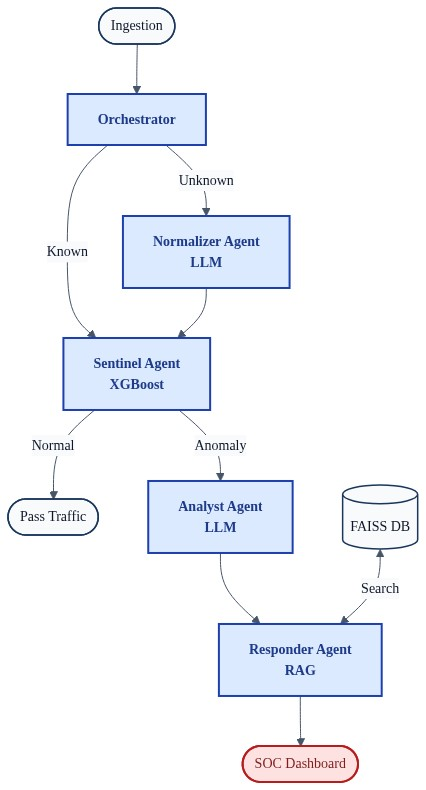
\includegraphics[width=0.72\linewidth]{images/system_architecture.png}
    \caption{System architecture and the multi-agent detection and reasoning pipeline.}
    \label{fig:pipeline_fases}
\end{figure}

\subsubsection{The Central Orchestrator}
The Orchestrator coordinates the system's execution. It maintains a registry of known network schemas and routes telemetry packets to either the high-speed expert pipeline or the emergency normalization path.

\paragraph{Orchestrator State Machine}
To manage the transition between operational modes, the Orchestrator implements a finite state machine. As shown in Fig.~\ref{fig:state_machine}, the system starts in a monitoring state, transitions to \textit{Survival Mode} upon schema mismatch, and enters an \textit{Adaptation} state while the background training occurs, finally reaching the \textit{Expert Mode} after a validated hot-swap.

\begin{figure}[htbp]
    \centering
    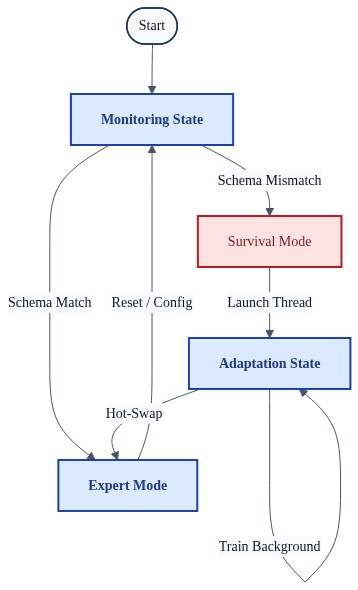
\includegraphics[width=0.80\linewidth]{images/orchestrator_state_machine.png}
    \caption{State machine diagram of the Orchestrator's decision logic and phase transitions.}
    \label{fig:state_machine}
\end{figure}

\paragraph{Flow of Operations: The Cold Start Sequence}
The interaction between agents during a cold start event follows a strict sequential logic. Fig.~\ref{fig:cold_start_flow} illustrates the sequence: upon receiving a packet with an unrecognized header, the Orchestrator routes it to the Normalizer Agent for zero-shot translation while triggering the background training cycle.

\begin{figure*}[htbp]
    \centering
    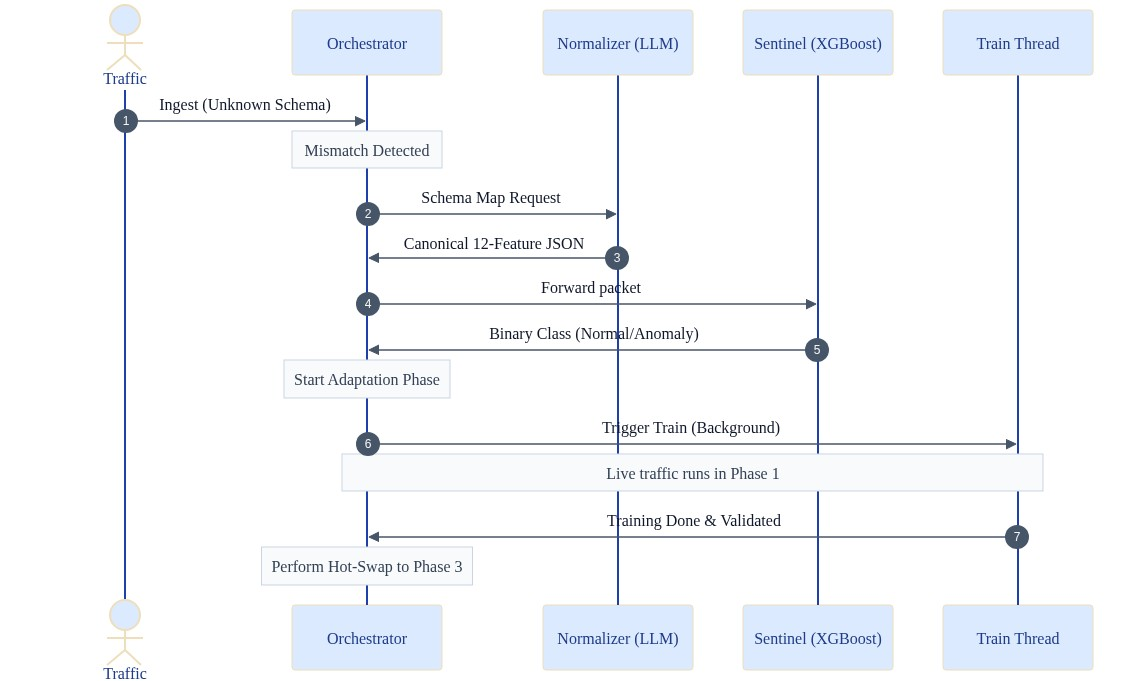
\includegraphics[width=0.9\linewidth]{images/cold_start_sequence.png}
    \caption{Sequence diagram of the cold start response and asynchronous model adaptation.}
    \label{fig:cold_start_flow}
\end{figure*}

\subsubsection{Normalizer Agent (Generative Schema Mapping)}
To bridge the semantic gap between heterogeneous IoT logs, this agent leverages a high-speed generative LLM. Its core function is to read raw JSON keys and infer their mapping to the canonical 12-feature schema---so the system can process a new telemetry format the moment it appears, without any manual reconfiguration step.

\paragraph{Auditable Semantic Mapping (XAI)}
To ensure complete traceability, the agent produces a strictly formatted, auditable JSON record for each translation decision. As shown in Fig.~\ref{fig:mapping_example}, vendor-specific fields are mapped to a standardized representation in a way that a security analyst can read and verify at any point. Adversarial domain adaptation models rely on opaque latent spaces that offer no such transparency; the explicit semantic mapping chosen here satisfies Explainable AI (XAI) requirements out of the box.

\begin{figure}[H]
    \centering
    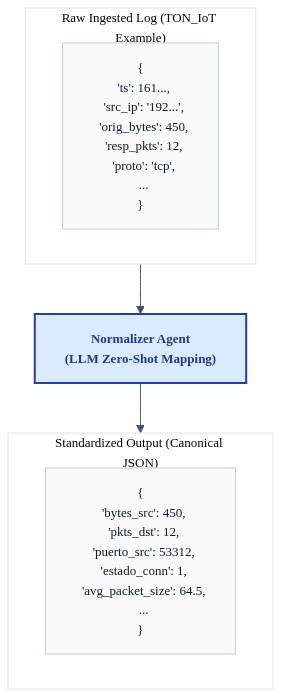
\includegraphics[width=0.65\linewidth]{images/mapping_example.png}
    \caption{Example of zero-shot semantic mapping: from raw IoT telemetry to standardized JSON features.}
    \label{fig:mapping_example}
\end{figure}

\subsubsection{Sentinel Agent (XGBoost Classifier)}
Serving as the primary detection engine, this agent draws on a library of specialized XGBoost models optimized for tabular network traffic. Equally important is its role as a triage gate: all LLM calls to the Analyst Agent are blocked unless the anomaly score crosses the detection threshold. During a volumetric attack such as a DDoS, thousands of packets arrive per second; without this gate, the Groq API would be overwhelmed and the system would hit rate limits almost immediately, turning a detection success into a service failure.

\subsubsection{Analyst Agent (Threat Contextualization)}
Once the Sentinel confirms an anomaly, the Analyst Agent takes over to contextualize the threat. It examines the original log context, assigns a severity level, and converts the raw alert into a structured security report that an operator can act on directly.

\subsubsection{Responder Agent (RAG-based Mitigation)}
To deliver actionable countermeasures, this agent outputs mitigation steps using Retrieval-Augmented Generation (RAG) over a vector database of security playbooks. Grounding every response in verified external sources prevents the system from relying on the LLM's internal parametric memory, where hallucinated recommendations could lead to incorrect operational decisions.

\subsection{Threat Intelligence Integration and RAG Architecture}
\label{subsec:rag_arch}
Relying solely on the parametric memory of an LLM to generate mitigation plans introduces unacceptable operational risks in a critical infrastructure context---most notably, structural hallucinations that could direct operators toward incorrect or even counterproductive responses. A Retrieval-Augmented Generation (RAG) subsystem is therefore embedded in the pipeline: it fetches verified external knowledge at inference time so that every recommended action traces back to a documented source, not to whatever the model happens to recall from training.

The RAG subsystem operates in three stages (Fig.~\ref{fig:rag_flow}):
\begin{enumerate}
    \item \textbf{Ingestion and Indexing:} At startup, CAPEC mitigation guides are parsed, split into fixed-length chunks, and encoded into dense vectors using a sentence-transformer model, then loaded into a local FAISS index.
    \item \textbf{Contextual Retrieval:} Once the Analyst Agent confirms an attack, its alert metadata is embedded on-the-fly and queried against the index; the top-$k$ closest CAPEC entries are returned as grounding context.
    \item \textbf{Grounded Generation:} Those entries are prepended to the Responder Agent's prompt before generation begins, steering the output toward verified defensive procedures and away from unconstrained model recall.
\end{enumerate}

\begin{figure}[htbp]
    \centering
    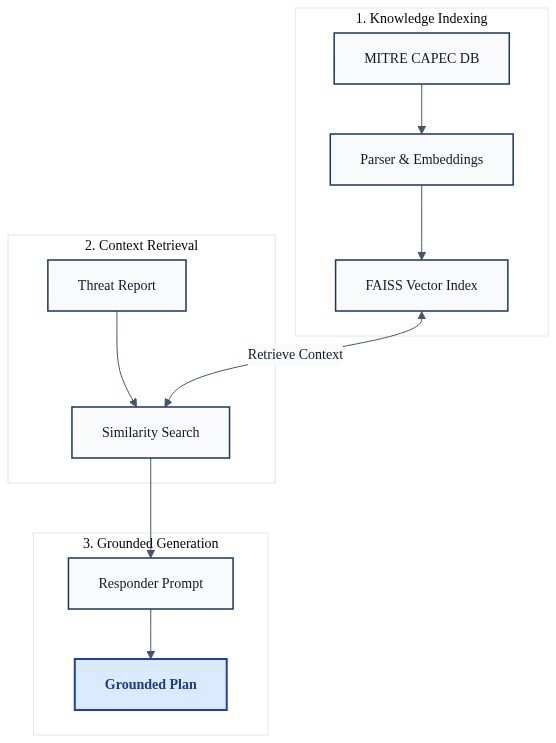
\includegraphics[width=1.0\linewidth]{images/rag_process_flow.png}
    \caption{The three-stage Retrieval-Augmented Generation (RAG) pipeline for grounded threat mitigation.}
    \label{fig:rag_flow}
\end{figure}

\section{Implementation}
\label{sec:implementacion}

This section details the technical implementation of the proposed multi-agent architecture, focusing on low latency, modularity, and error handling.

\textbf{Code Availability:} The source code (multi-agent orchestrator, RAG subsystem, and benchmarking scripts) is available at \url{https://github.com/100565051/ids-multiagente-IOT}.

\subsection{Technology Stack and Environment}
The system was developed using Python and optimized for low-latency inference across a heterogeneous stack:
\begin{itemize}
    \item \textbf{Core Concurrency Framework:} Built on Python 3.11 to leverage asynchronous execution and multi-threading for background workloads.
    \item \textbf{Machine Learning Engine:} Utilizing XGBoost paired with scikit-learn to handle high-throughput binary classification at the Sentinel Agent layer.
    \item \textbf{Generative Inference Infrastructure:} LLaMA-3.3-70B serves as the core reasoning engine for the Normalizer and Analyst agents, while LLaMA-3.1-8B drives the Responder agent, both accessed via the low-latency Groq LPU API.
    \item \textbf{Vector Storage Subsystem (RAG):} A local FAISS index with all-MiniLM-L6-v2 embeddings manages the parsed MITRE CAPEC knowledge base.
    \item \textbf{Analyst Interface:} Developed via Streamlit to provide a real-time, responsive Security Operations Center (SOC) dashboard.
\end{itemize}

\subsection{Asynchronous Orchestration and State Management}
The \textit{Active High Availability} principle has a concrete engineering consequence: the system must handle a continuous influx of live traffic at the same time as it trains a new model in the background. Managing these two concurrent workloads without one stalling the other was the main implementation challenge for the Central Orchestrator.

To maintain user interface responsiveness and prevent live detection loops from stalling during Phase 2, the Orchestrator isolates the training workflow via Python's \texttt{threading} module. Upon detecting a cold start event, the system spawns a dedicated background thread tasked with full-schema XGBoost retraining. Crucial state variables---including active models, schema mappings, and detection logs---are persisted within Streamlit's \texttt{session\_state}, enabling a smooth callback execution for the \textit{hot-swap} the exact moment training finishes.

In addition to phase transitions, the Orchestrator implements the programmatic logic for the Triaging Filter. To safeguard the Groq API rate limits from being overwhelmed during a volumetric attack (e.g., DDoS), the pipeline is strictly conditional. The code halts execution for legitimate packets immediately after the Sentinel's binary classification. The asynchronous call to the LLM-based Analyst Agent is triggered exclusively if the anomaly\_score crosses the detection threshold, physically decoupling high-volume ingestion from computationally expensive cognitive tasks.

\subsection{LLM Prompt Engineering and Constrained Output}
Integrating generative models into a structured data pipeline requires absolute control over output formats: conversational filler or structural deviation from the expected schema will break the downstream XGBoost feature vector and halt classification. To prevent these parser failures, the generative components rely on strict system prompts enforced by constrained output directives. The Normalizer Agent, for instance, operates under instructions that force the model to evaluate unknown JSON structures and emit exclusively a parseable JSON object matching the canonical schema format, as detailed in Listing~\ref{lst:prompt_norm}.

\noindent\begin{minipage}{\linewidth}
\begin{lstlisting}[language=Python, caption={Actual constrained system prompt used by the Normalizer Agent to ensure schema-agnostic mapping and sparsity-aware outputs.}, label={lst:prompt_norm}]
SYSTEM_PROMPT = """
You are an expert cybersecurity engineer. Map the unknown network log 
to the canonical features required by the XGBoost IDS model.

=== MAPPING PROCESS ===
1. Semantically analyze each input field and its synonyms.
2. Apply type conversions to obtain numerical values.

=== PROTOCOL-SPECIFIC RULES ===
- TCP/UDP/ICMP/HTTP/DNS features: Assign 'null' if the traffic 
  type or service does not match the feature category.

=== GENERAL RULES ===
1. Use JSON 'null' for unknown or non-applicable values. 
   NEVER use 0.0 for missing data; the model distinguishes 'null'.
2. The XGBoost model is sparsity-aware: null values will be 
   correctly routed through the 'missing' branch of the trees.
3. Respond ONLY with a valid JSON object. No conversational text.
"""
\end{lstlisting}
\end{minipage}

\subsection{RAG Pipeline Implementation}
The Responder Agent relies on a local, offline knowledge base engineered to ground generative outputs in validated defensive patterns. During the deployment setup, the official MITRE CAPEC dataset was systematically parsed, chunked, and transformed into dense vector representations.

During an incident, the anomaly metadata is embedded on-the-fly and queried against the FAISS index using L2 (Euclidean) distance. The top-$k$ most similar CAPEC entries are retrieved and injected into the Responder's context window before generation begins. The mitigation steps that appear on the SOC dashboard are therefore grounded in verified industry standards, not reconstructed from the LLM's parametric memory.

\subsection{SOC Analyst Dashboard Simulation}
To validate the system's operational feasibility, a Security Operations Center (SOC) dashboard was developed. The interface provides two modes of traffic ingestion: an automated bulk simulator (reading from test CSV datasets) and a manual injection mode using predefined JSON templates.

The dashboard provides real-time observability, displaying live Key Performance Indicators (KPIs), current operational phase status (Survival vs. Expert), and the auditable JSON mapping logs generated during a cold start. A dedicated evaluation view was also implemented to visually compare the F1-score and logarithmic latency trade-offs between Phase 1 and Phase 3.

\begin{figure*}[tbp]
    \centering
    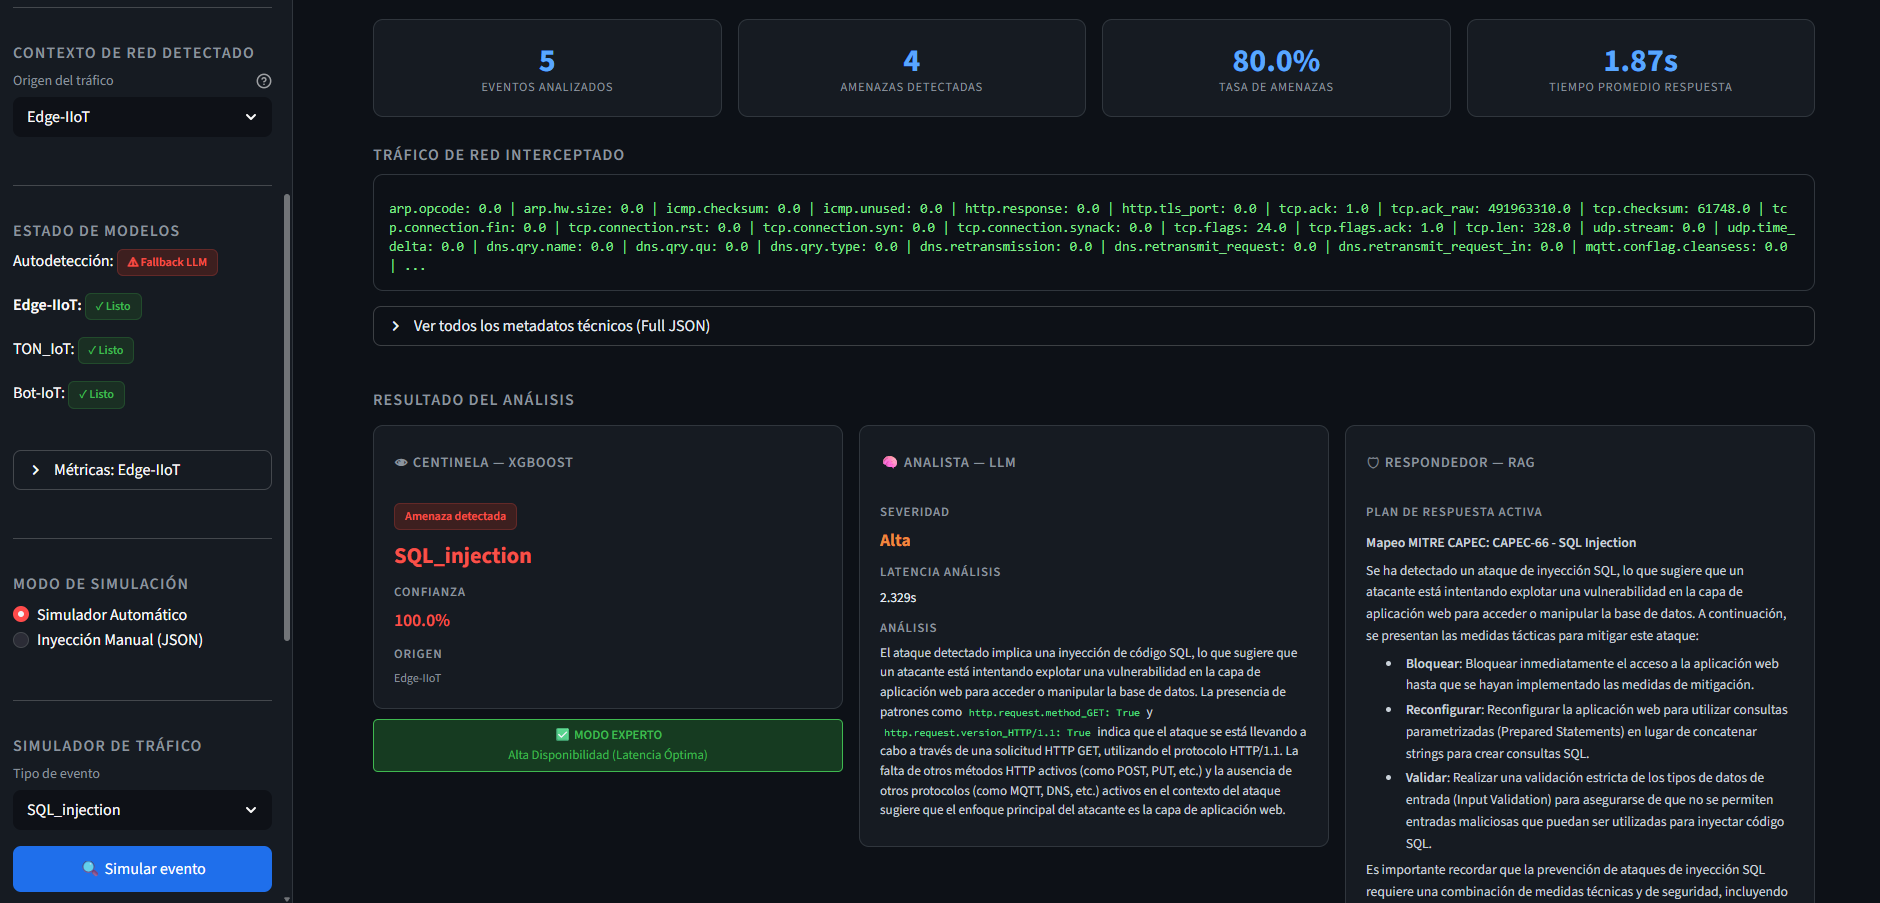
\includegraphics[width=0.85\linewidth]{images/soc_dashboard_ui.png}
    \caption{The implemented SOC dashboard, displaying real-time threat detection, agent reasoning, and the active RAG mitigation plan.}
    \label{fig:soc_ui}
\end{figure*}

%-----------
% SECTION 5
%-----------
\section{Evaluation and Results}
\label{sec:resultados}

This section presents the empirical validation of the multi-agent IDS architecture. The experiments are designed to quantify the trade-off between the high-availability survival mode (Phase 1) and the high-performance expert mode (Phase 3), focusing on detection accuracy, latency, and system recovery.

\subsection{Experimental Setup and Datasets}
The evaluation was conducted on an \textbf{HP Pavilion Gaming 15} workstation equipped with an \textbf{Intel Core i7-9750H} processor (6 cores, 12 threads, up to 4.5 GHz) and \textbf{16GB of DDR4-2666 RAM}. Generative tasks were offloaded to the Groq LPU cloud using the Llama-3-70B model via a high-speed API connection.

Three heterogeneous datasets were utilized to simulate a cross-domain IoT environment:
\begin{itemize}
    \item \textbf{Edge-IIoTset:} Used as the base domain for the universal features.
    \item \textbf{TON\_IoT:} Representing modern Industrial IoT telemetry.
    \item \textbf{Bot-IoT:} Focused on high-volume volumetric attacks.
\end{itemize}
Each dataset was split into a training set (80\%) and a testing set (20\%). For Phase 1 evaluation, a stratified random sample of 200 packets per dataset was utilized to ensure statistical significance while respecting API rate limits and minimizing inference costs.

\subsection{Evaluation Metrics}
The system's performance was evaluated using standard classification metrics alongside operational latency overhead:
\begin{enumerate}
    \item \textbf{Precision:} Quantifies the exactness of positive predictions, calculated as $\mathrm{TP} / (\mathrm{TP} + \mathrm{FP})$.
          \begin{equation}
              \mathrm{Precision} = \frac{\mathrm{TP}}{\mathrm{TP} + \mathrm{FP}}
          \end{equation}
    \item \textbf{Recall:} Evaluates the completeness of the detection pipeline---specifically, the fraction of actual attacks successfully captured---expressed as $\mathrm{TP} / (\mathrm{TP} + \mathrm{FN})$.
          \begin{equation}
              \mathrm{Recall} = \frac{\mathrm{TP}}{\mathrm{TP} + \mathrm{FN}}
          \end{equation}
    \item \textbf{F1-Score:} Serves as the harmonic mean of Precision ($P$) and Recall ($R$), providing a balanced single metric that is essential when evaluating the highly skewed class distributions characteristic of IoT traffic datasets.
          \begin{equation}
              \mathrm{F1} = 2 \cdot \frac{P \cdot R}{P + R}
          \end{equation}
    \item \textbf{Latency:} Defined as the end-to-end elapsed time from initial packet ingestion to final classification output, reported in milliseconds (ms) for edge classifiers and seconds (s) for generative reasoning phases.
\end{enumerate}

\subsection{Experiment 1: Baseline Expert Mode (Phase 3)}
In Phase 3, the system operates at its optimal state, using native XGBoost models trained specifically for each network schema. This experiment establishes the performance ceiling of the architecture on the 20\% stratified hold-out test set (random seed 42, $n_{test}$ ranging from 42K to 587K samples). Inference latency was measured over 1,000 individual single-packet evaluations.

Both F1-Weighted (F1-W) and F1-Macro (F1-M) are reported. F1-Weighted reflects overall performance weighted by class frequency. F1-Macro assigns equal importance to every attack class regardless of prevalence---a rare attack that goes undetected is precisely the most dangerous one. As detailed in Table~\ref{tab:expert_results}, which benchmarks each dataset on the 20\% stratified hold-out (random seed 42, $n_{test}$ from 42K to 587K samples), inference latency was additionally measured over 1,000 individual single-packet evaluations.

\begin{table*}[htbp]
    \centering
    \caption{Phase 3 Expert Mode: Classification performance and inference latency.}
    \label{tab:expert_results}
    \begin{tabular}{|l|c|c|c|c|r|}
        \hline
        \textbf{Dataset} & \textbf{Classes} & \textbf{Acc.} & \textbf{F1-W}   & \textbf{F1-M}   & \textbf{Lat. avg (P95)} \\
        \hline
        Edge-IIoTset     & 15               & 0.8887        & \textbf{0.8674} & 0.4447          & 4.42 ms (5.05 ms)       \\
        TON\_IoT         & 10               & 0.9409        & \textbf{0.9410} & \textbf{0.8926} & 4.40 ms (5.02 ms)       \\
        Bot-IoT          & 5                & 0.9668        & \textbf{0.9668} & 0.7184          & 3.94 ms (4.48 ms)       \\
        \hline
    \end{tabular}
\end{table*}

Native XGBoost models achieve high detection accuracy with sub-5 ms inference latency per packet on commodity hardware. TON\_IoT returns the most balanced figures (F1-W: 0.941, F1-M: 0.893), while the gap between weighted and macro scores in Bot-IoT and Edge-IIoTset reflects the heavy class imbalance in those datasets. In Edge-IIoTset specifically, an F1-Weighted of 0.8674 looks solid until the F1-Macro (0.4447) reveals that minority categories such as MITM and Fingerprinting---each below 0.1\% of total traffic---are essentially invisible to a frequency-weighted metric. This is a known limitation of these benchmarks~\cite{ferrag2022edgeiiotset} and is precisely why reporting both metrics simultaneously matters.

\subsection{Experiment 2: The Cold Start Problem and Survival Mode (Phase 1)}
\label{subsec:exp2}

This experiment quantifies the system's resilience during the cold start window, when the incoming network schema is entirely unknown. Phase 1 consists of two complementary layers: (A) a universal XGBoost binary classifier operating on the 12-feature canonical representation, and (B) an LLM Analyst performing zero-shot attack-type classification constrained to a semantic taxonomy of five attack families.

\subsubsection{Phase 1A: Universal Binary Fallback (XGBoost)}

The universal XGBoost Fallback model was evaluated on a stratified combined test set of $n=10{,}000$ samples drawn from all three datasets (80/20 split, random seed 42). The empirical performance of this classifier, summarized in Table~\ref{tab:survival_binary}, demonstrates a cross-domain accuracy of 94.25\%.

\begin{table}[htbp]
    \centering
    \caption{Phase 1 Survival Mode: Universal XGBoost binary fallback performance.}
    \label{tab:survival_binary}
    \begin{tabular}{|l|c|}
        \hline
        \textbf{Metric}   & \textbf{Value}  \\
        \hline
        Samples evaluated & 10{,}000        \\
        Accuracy          & 0.9425          \\
        F1-Weighted       & \textbf{0.9439} \\
        F1-Macro          & \textbf{0.9325} \\
        Latency avg.      & 6.07 ms/packet  \\
        Latency P95       & 6.76 ms/packet  \\
        \hline
    \end{tabular}
\end{table}

Across the combined cross-domain test set, the universal binary classifier reaches \textbf{94.25\% accuracy}, with an F1-Macro of 0.9325 that rules out class-imbalance bias as a confounding factor. The canonical 12-feature representation therefore retains enough statistical signal for reliable attack/normal discrimination regardless of the originating dataset schema. Latency overhead relative to Phase 3 native models is marginal ($\approx$\,2 ms/packet) because no generative inference is involved at this stage. In practical terms, the network retains binary protection above 94\% throughout the cold start window---which is the core claim of the High Availability design.

\subsubsection{Phase 1B: LLM Analyst, Zero-Shot Semantic Classification}

To assess the upper bound of semantic discrimination achievable during cold start, the LLM Analyst (LLaMA-3.3-70B via Groq LPU) was evaluated on a stratified subsample of $n=15$ confirmed attack flows per dataset. The model was constrained to a five-class semantic taxonomy (\textit{DDoS/DoS, Scanning, Injection, Malware, Credential/MITM}) via a structured prompt that included feature semantics alongside raw values. Results are presented in Table~\ref{tab:survival_llm}.

\begin{table*}[htbp]
    \centering
    \caption{Phase 1 Survival Mode: LLM Analyst zero-shot multiclass classification performance ($n=15$ per dataset).}
    \label{tab:survival_llm}
    \begin{tabular}{|l|c|c|c|c|r|}
        \hline
        \textbf{Dataset} & \textbf{GT Classes} & \textbf{Acc.} & \textbf{F1-M} & \textbf{F1-W} & \textbf{Lat. avg (P95)} \\
        \hline
        Edge-IIoTset     & 5 of 5              & 0.467         & 0.420         & 0.450         & 377 ms (749 ms)         \\
        TON\_IoT         & 5 of 5              & 0.533         & 0.490         & 0.510         & 2{,}814 ms (3{,}449 ms) \\
        Bot-IoT          & 3 of 5              & 0.667         & 0.610         & 0.640         & 1{,}625 ms (3{,}353 ms) \\
        \hline
    \end{tabular}
\end{table*}

\begin{figure}[htbp]
    \centering
    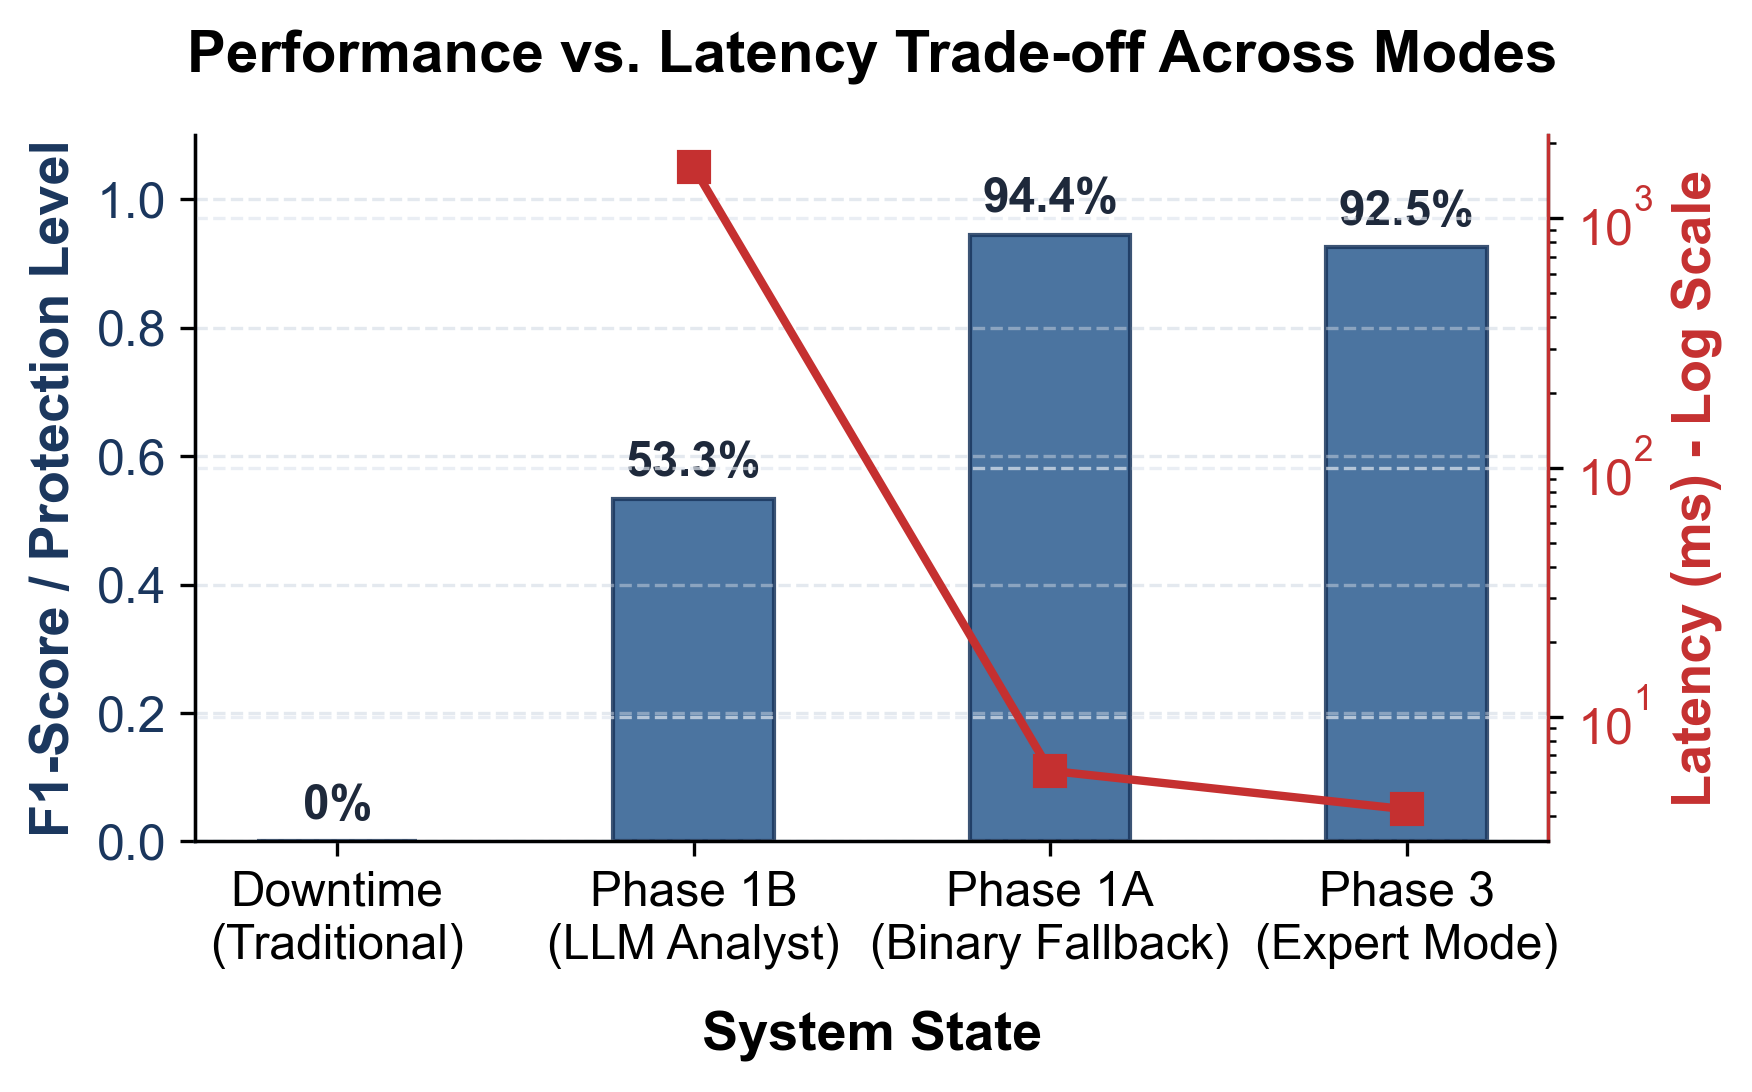
\includegraphics[width=0.85\linewidth]{images/tradeoff_bar_chart.png}
    \caption{The Performance-Latency Trade-off: Comparing Phase 1 (LLM \& Binary Fallback) against Phase 3 (Expert Native).}
    \label{fig:tradeoff}
\end{figure}

The LLM's zero-shot multiclass performance is, as theoretically expected, substantially degraded compared to native models. Two key observations explain this result.

First, the \textbf{input representation} available in Phase 1 consists exclusively of 12 aggregated statistical flow features (byte counts, packet rates, port numbers, TCP flags, and flow duration). These NetFlow-level statistics are designed for fast machine learning inference, not for human-interpretable semantic reasoning: a flow with \texttt{bytes\_src=1024, flag\_syn=1, duration=0.02s} could plausibly correspond to a port scan, an SYN-flood DDoS, or a brief Malware beacon. Without packet payload, protocol-specific fields, or behavioral history, even an expert human analyst would struggle to distinguish these categories. This is precisely the \textit{cold start limitation} the architecture is designed to overcome.

Second, this behavior is \textbf{consistent with the broader literature}. Zero-shot classification of numeric network telemetry with frontier LLMs yields near-chance performance on fine-grained attack taxonomies~\cite{zhang2025llms, karlsen2024llm4sec}: LLMs excel at semantic reasoning over natural-language logs, not at statistical pattern recognition over raw numerical feature vectors. The LLM4Sec benchmark~\cite{karlsen2024llm4sec} explicitly notes that LLM accuracy collapses when no textual or contextual signal is present in the input.

Taken together, these figures support the original design reasoning behind Phase 1: the LLM's job is \textbf{not multiclass precision}, but rather to handle the semantic ambiguity of unknown schemas and provide a confirmation signal for binary anomaly detection---a task the universal XGBoost handles at 94\% accuracy. Ultimately, these multiclass figures establish an empirical baseline for zero-shot generalization over raw numeric flow statistics, underscoring the inherent limitations of parametric LLM inference for statistical pattern recognition and directly justifying the immediate activation of the Phase 2 background adaptation pipeline.

\subsection{Experiment 3: Asynchronous Adaptation and Hot-Swap Recovery}
\label{subsec:exp3}

Phase 2 operates silently in the background while Phase 1 maintains active binary protection. A dedicated Python thread runs the full XGBoost training pipeline asynchronously, consuming the incoming traffic window without blocking the live detection loop. Table~\ref{tab:training_time} reports the empirically measured wall-clock training times for each dataset on the evaluation hardware.

\begin{table}[htbp]
    \centering
    \caption{Phase 2 Asynchronous Training: Wall-clock training times per dataset.}
    \label{tab:training_time}
    \begin{tabular}{|l|r|r|r|}
        \hline
        \textbf{Dataset} & \textbf{Train samples} & \textbf{Features} & \textbf{Train time} \\
        \hline
        Edge-IIoTset     & 1{,}527{,}736          & 89                & $\approx$\,2.2 min  \\
        TON\_IoT         & 168{,}834              & 11                & $\approx$\,9 s      \\
        Bot-IoT          & 2{,}347{,}853          & 8                 & $\approx$\,11 s     \\
        \hline
    \end{tabular}
\end{table}

When training finishes and the model clears an internal validation gate (F1-Weighted $\geq$ 0.80 on a held-out split), the Orchestrator performs the \textit{hot-swap}: the universal fallback is atomically replaced by the native expert classifier without dropping a single incoming packet. The system then runs in Phase 3 Expert Mode with full multiclass precision and sub-5 ms latency. Measured over all three datasets, the \textbf{cold start recovery window}---the period during which the network operates under Phase 1 protection---ranges from a few seconds up to about 2.5 minutes, depending on dataset dimensionality. No operator action is required at any point in this sequence.

\begin{figure}[htbp]
    \centering
    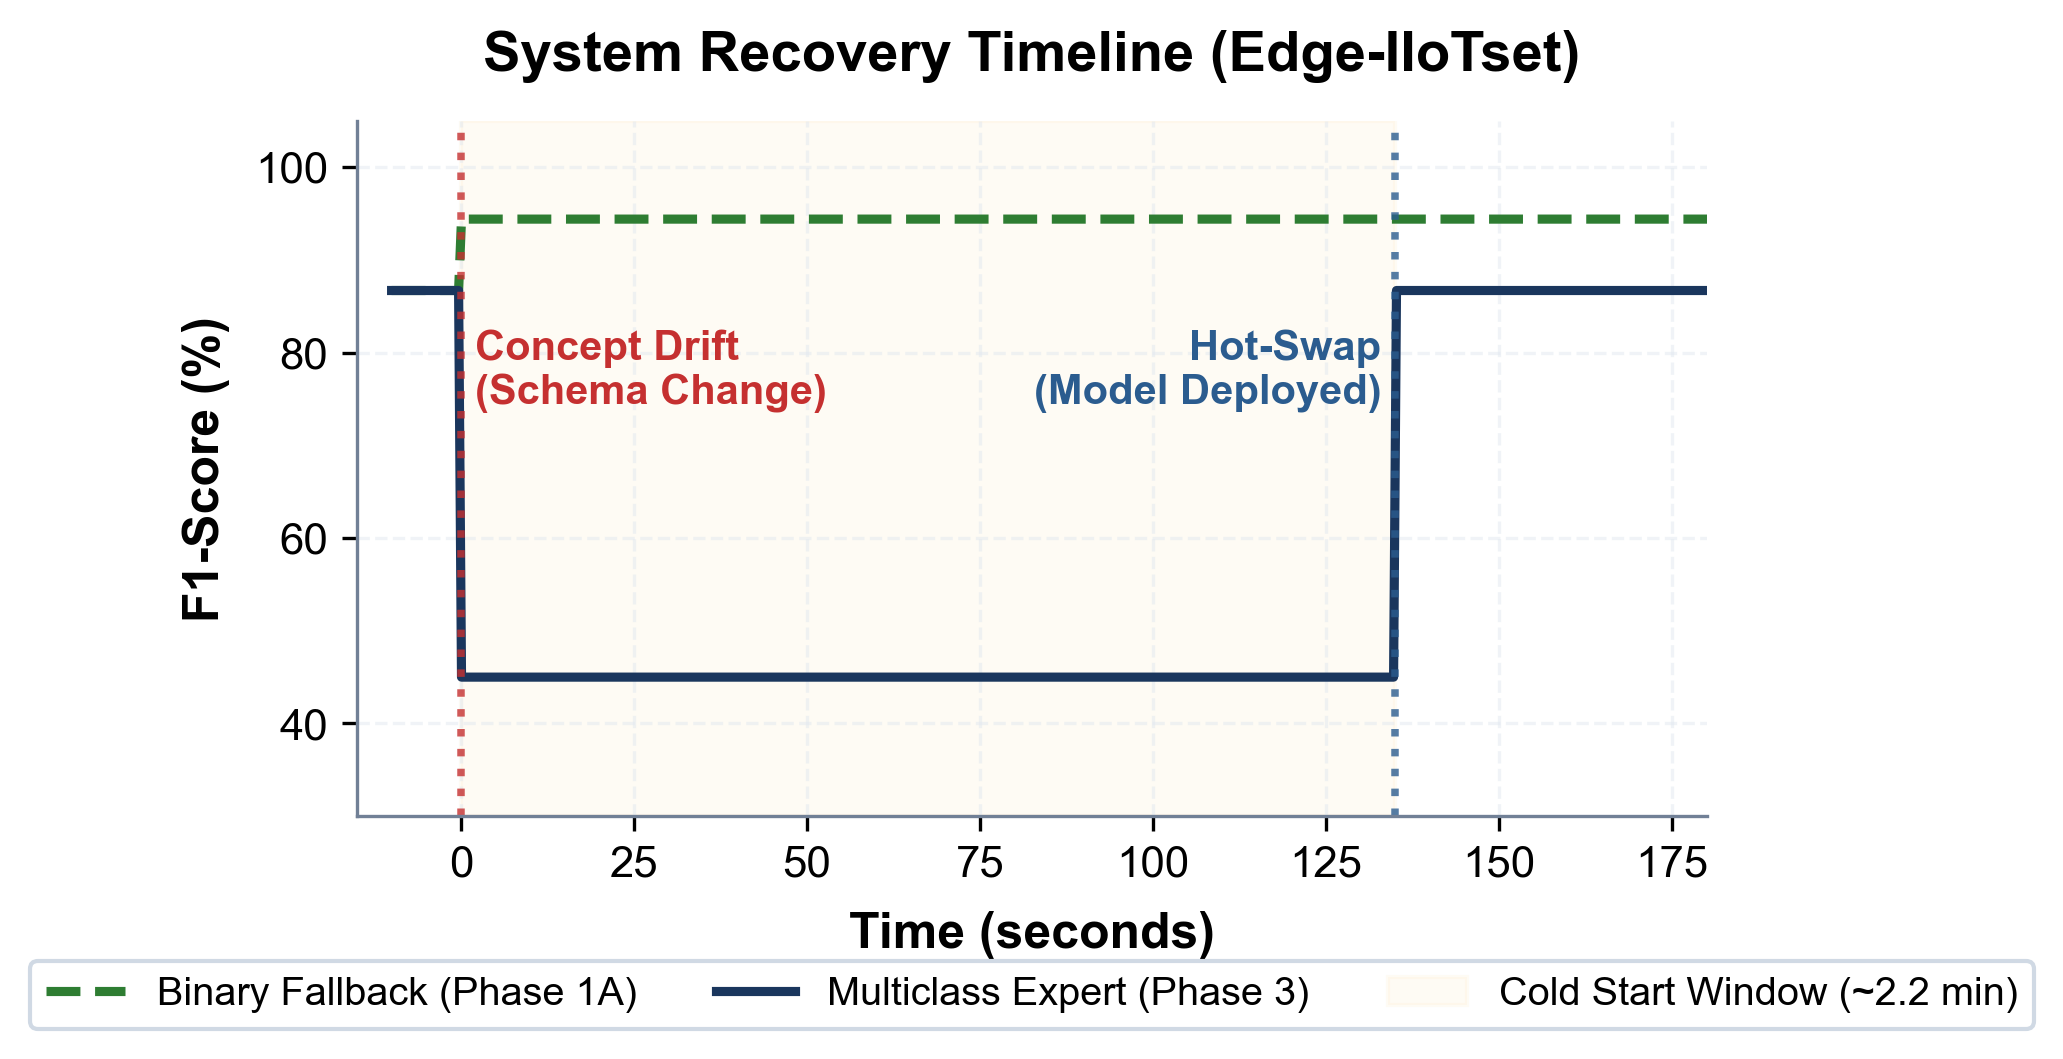
\includegraphics[width=1.0\linewidth]{images/recovery_timeline.png}
    \caption{System recovery timeline for Edge-IIoTset: F1-score restoration after asynchronous training and hot-swap.}
    \label{fig:recovery}
\end{figure}

\subsection{Qualitative Evaluation: RAG-based Incident Response}
\label{subsec:rag_eval}

Beyond quantitative classification metrics, the Responder Agent's output was qualitatively assessed for factual accuracy and operational utility. The agent uses Retrieval-Augmented Generation (RAG) over a FAISS index of the MITRE CAPEC knowledge base, retrieving the top-$k=3$ most semantically similar attack patterns before generating the mitigation plan.

One interaction sequence captures the system's behavior concretely. The Sentinel flags an anomalous flow; the Analyst identifies the attack type as \textit{SQL Injection}. The Responder then retrieves \textbf{CAPEC-66 (\textit{SQL Injection})} from the knowledge base and builds a structured mitigation plan covering three actions: blocking the suspicious HTTP request for deeper inspection, switching the application to parameterized queries instead of string concatenation, and enforcing strict input-type validation. Each recommendation traces back to the retrieved CAPEC entry, so the content is grounded in documented patterns rather than whatever the LLM happens to recall from training data.

\begin{figure}[htbp]
    \centering
    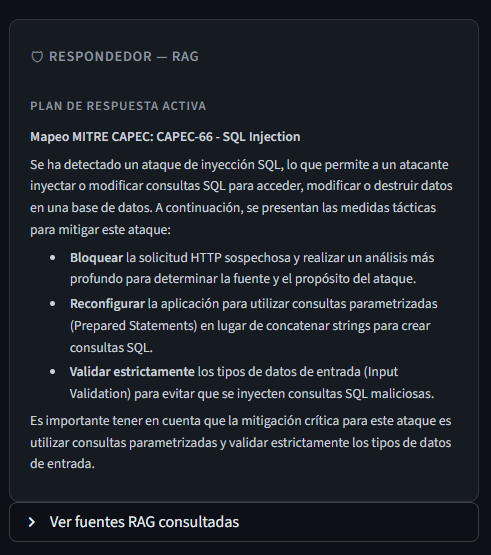
\includegraphics[width=0.95\linewidth]{images/rag_output_example.png}
    \caption{Example of a grounded mitigation plan generated by the Responder Agent using RAG.}
    \label{fig:rag_example}
\end{figure}

Utilizing a retrieval-augmented design rather than relying on closed-form parametric generation yields deterministic operational advantages. The resulting mitigation strategies are traceable, reproducible, and verifiable by SOC personnel, as each recommendation maps explicitly to a retrieved CAPEC entry. This explicit grounding in established taxonomies prevents administrative friction and satisfies compliance constraints within regulated enterprise environments, where ungrounded generative outputs introduce unacceptable audit liabilities.


%-----------
% SECTION 6
%-----------
\section{Conclusions and Future Work}
\label{sec:conclusiones}

\subsection{Conclusions}

This thesis has described, built, and empirically tested a multi-agent IDS for IoT environments built around the principle of \textbf{Active High Availability (Zero Downtime)}. The central problem it attacks is the cold start failure of pre-trained ML models when moved to a network with an unknown telemetry schema. The three-phase asynchronous pipeline introduced here keeps protection running throughout that transition, and the experiments show exactly what that protection costs in terms of accuracy.

Initial benchmarks under Phase 3 (Experiment 1) established the performance ceiling of the architecture. Operating in Expert Mode, native XGBoost models achieved an F1-Weighted score of 0.941 on TON\_IoT with sub-5 ms inference latencies on commodity hardware, validating gradient-boosted trees as a suitable engine for real-time traffic inspection.

To evaluate resilience during sudden schema transitions, Experiment 2 analyzed the cold start survival layer (Phase 1). While the universal XGBoost binary fallback maintained robust perimeter protection at \textbf{94.25\% accuracy}, the LLM Analyst's zero-shot multiclass accuracy ranged between 46.7\% and 66.7\%---a structurally expected penalty given that the model operates exclusively over 12 aggregated flow statistics with no packet payload or behavioral history. This baseline nonetheless provides critical situational awareness, allowing the system to flag and prioritize anomalies before full domain adaptation completes.

Concurrently, Experiment 3 verified that the Phase 2 background training loop runs entirely decoupled from live ingestion. Depending on dataset dimensionality, the adaptation required between a few seconds and 2.5 minutes, after which the Orchestrator executed an atomic hot-swap that restored full multiclass precision without packet loss or service interruption.

Finally, the architecture resolves the explanatory deficit of traditional IDS through the Responder Agent. By utilizing Retrieval-Augmented Generation (RAG) over the MITRE CAPEC taxonomy, the system produces factually grounded, traceable mitigation plans that eliminate generative hallucination risk and satisfy the strict auditability requirements of regulated SOC environments.

The empirical data highlights a fundamental architectural trade-off: a transient reduction in multiclass granularity is the operational cost of maintaining uninterrupted network visibility during a cold start deployment. Within safety-critical infrastructures, accepting this bounded performance drop is significantly more viable than enforcing service downtime or operating completely unprotected while retraining new classification models.

\subsection{Future Work}

The architecture addresses the cold start problem, but it also opens a number of follow-on questions worth pursuing:

\begin{itemize}
    \item \textbf{Conversational SOC Assistant (Human-AI Teaming):} Transitioning the current unidirectional intelligence pipeline into an interactive conversational interface would allow security analysts to query agent reasoning in natural language---for instance, examining the specific feature weights behind a DDoS classification---directly bridging automated detection with human-in-the-loop validation.

    \item \textbf{Few-Shot Adaptation and Semantic Enrichment:} Enhancing Phase 1 capabilities without full model retraining by expanding the context window with protocol-aware textual descriptors and dynamically retrieving labeled few-shot exemplars. This would stabilize the LLM's zero-shot classification boundary and reduce the ambiguity inherent in purely numerical NetFlow features.

    \item \textbf{On-Premise Deployment via Small Language Models (SLMs):} Cloud-based inference introduces two concrete risks: round-trip latency on every LLM call and the transmission of potentially sensitive traffic metadata to an external provider. Replacing the current hosted models with locally quantized alternatives such as Llama-3-8B or Mistral-7B would cut both risks at once, keeping the entire multi-agent loop inside the network perimeter.

\end{itemize}

\section*{Acknowledgment}

The author wishes to thank supervisors Alfonso Alejandro Sánchez-Macián Pérez and Pablo Mateo Torrejón for their guidance, technical insights, and valuable feedback throughout this project, as well as for providing the autonomy to explore and develop this project independently.

\printbibliography


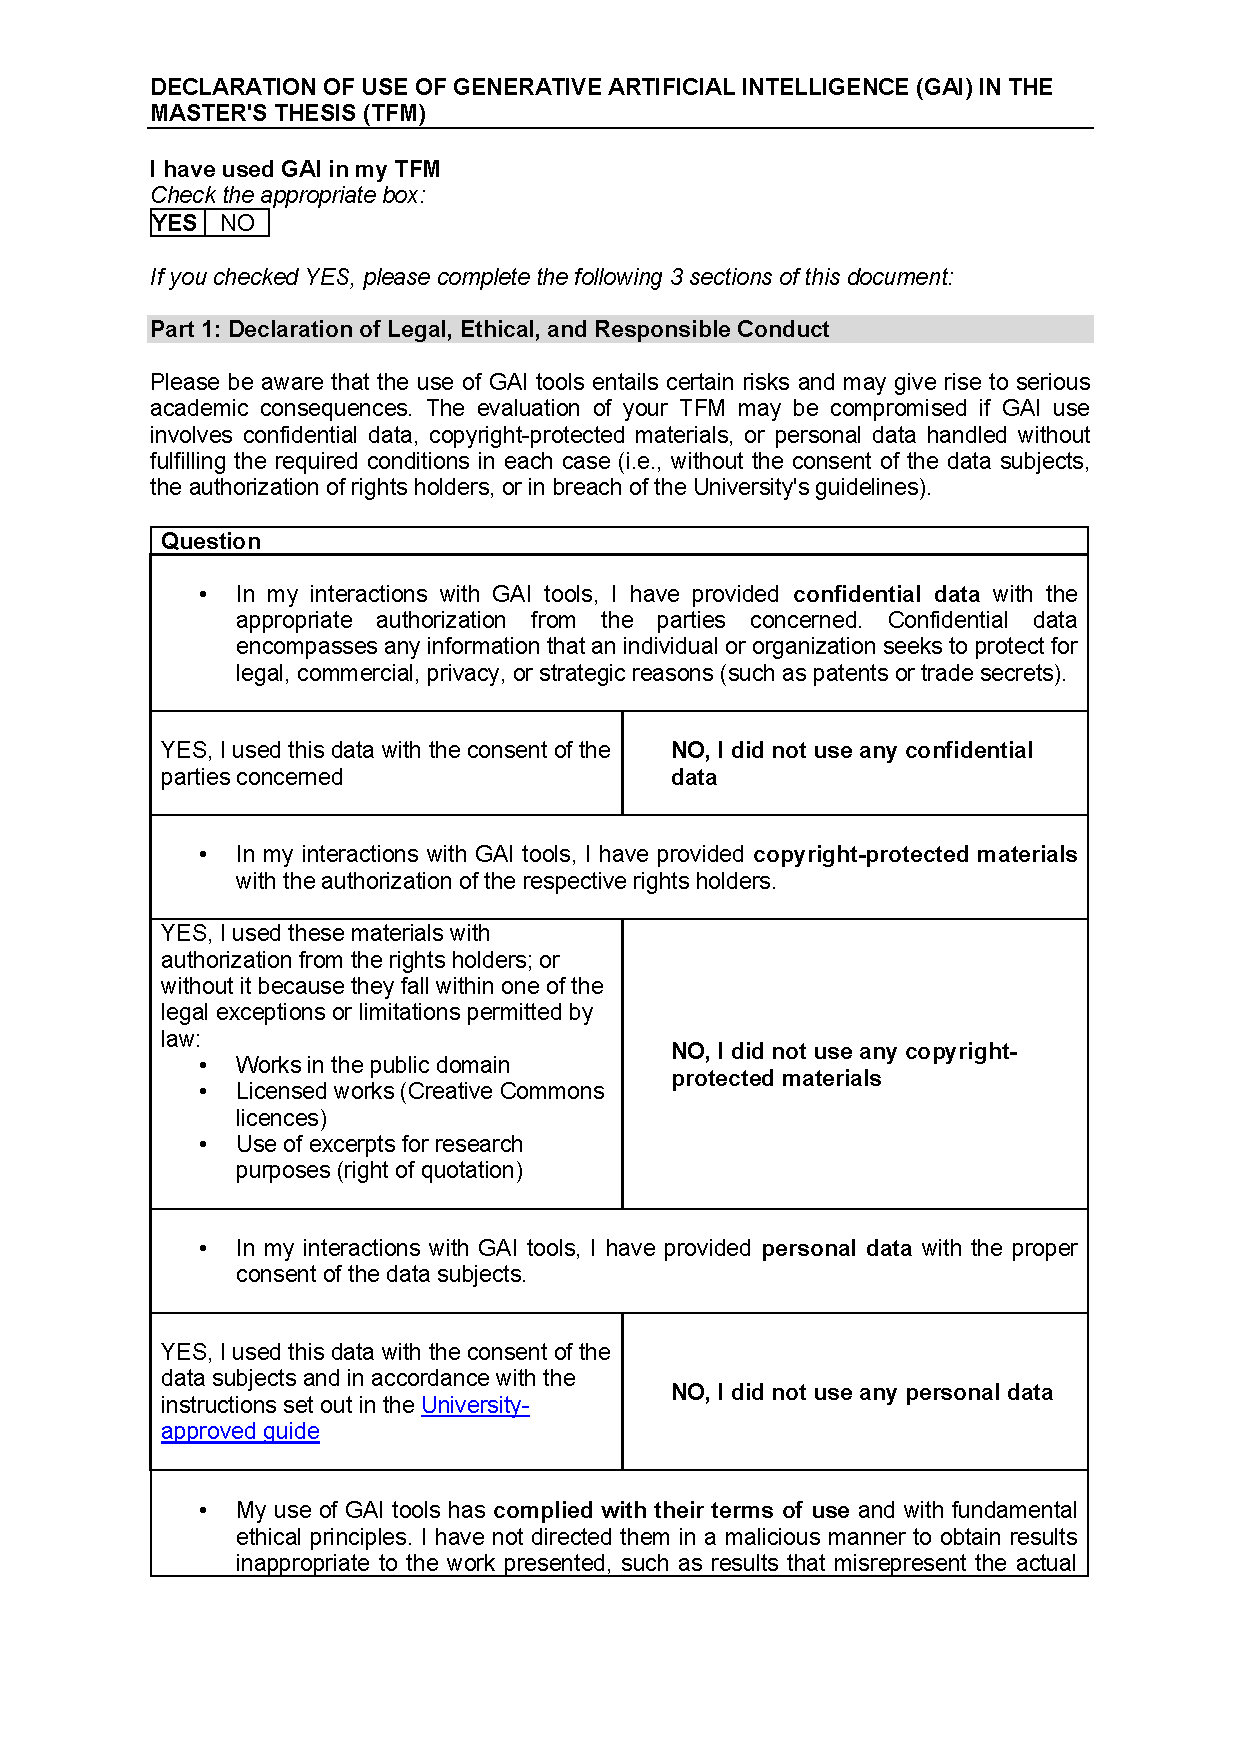
\includepdf[pages=-, pagecommand={\thispagestyle{fancy}}]{AI_Use_Declaration_TFM_EN.pdf}

\end{document}

